  \documentclass{article}

% if you need to pass options to natbib, use, e.g.:
% \PassOptionsToPackage{numbers, compress}{natbib}
% before loading nips_2017
%
% to avoid loading the natbib package, add option nonatbib:
% \usepackage[nonatbib]{nips_2017}

\usepackage{nips_2017}
\usepackage{etoolbox}
\usepackage{graphicx}
\usepackage{subcaption}
\patchcmd{\thebibliography}{\section*{\refname}}{}{}{}

% to compile a camera-ready version, add the [final] option, e.g.:
% \usepackage[final]{nips_2017}

\usepackage[utf8]{inputenc} % allow utf-8 input
\usepackage[T1]{fontenc}    % use 8-bit T1 fonts
\usepackage{hyperref}       % hyperlinks
\usepackage{url}            % simple URL typesetting
\usepackage{booktabs}       % professional-quality tables
\usepackage{amsfonts}       % blackboard math symbols
\usepackage{nicefrac}       % compact symbols for 1/2, etc.
\usepackage{microtype}      % microtypography

\title{Style Transfer for Music}

\author{
  Anshu Aviral\\
%   Carnegie Mellon University\\
  \texttt{aanshu@andrew.cmu.edu} \\
  %% examples of more authors
  \And
  Justin Wang\\
  %   Carnegie Mellon University\\
  \texttt{jcwang1@andrew.cmu.edu} \\
  \And
  Sivaprasad Sudhir\\
%   Carnegie Mellon University\\
  \texttt{sivapras@andrew.cmu.edu} 
}

\begin{document}
% \nipsfinalcopy is no longer used

\maketitle
% \begin{abstract}
%   The abstract paragraph should be indented \nicefrac{1}{2}~inch
%   (3~picas) on both the left- and right-hand margins. Use 10~point
%   type, with a vertical spacing (leading) of 11~points.  The word
%   \textbf{Abstract} must be centered, bold, and in point size 12. Two
%   line spaces precede the abstract. The abstract must be limited to
%   one paragraph.
% \end{abstract}

\section{Introduction}

In recent years, deep learning techniques have been applied to a variety of problems on visual data.  
One such application has been that of artistic style transfer.
At a high level, artistic style transfer has the following goal: given image A and a work by artist B, generate a rendering of A's content in the style of artist B.
Though loss-functions are used for training, the algorithm's success is ultimately evaluated subjectively, by asking: does the output image seem to compellingly reflect artistic style transfer?
For example, if the output image is in the style of B but also contains much of B's content, this would not be a totally satisfactory solution.

We seek to explore the problem of style transfer between musical pieces.
The field of machine learning for musical data is relatively less explored than that for visual data. We think working on style transfer will help us understand not only which machine learning methods for visual data can be effectively applied for musical data, but also which aspects of musical data are distinctive enough to require new ideas.

Given the relatively small body of work on machine learning for musical data, for tractability purposes, we restrict our focus to a narrower definition of style transfer.
Rather than blending the content of an arbitrary song A with the style of an arbitrary musical artist B, we'll simply seek to do instrument-to-instrument style transfer.
That is, given input audio of instrument A playing some notes and a target instrument B,
we'll seek to generate output audio that sounds as if instrument B were playing the same notes as A.
We are simplifying the general notion of musical content to just be a series of notes,
and the general notion of musical style to just be the timbral qualities of an instrument.
Similar to artistic style transfer, the ultimate evaluation of a successful instrument-to-instrument algorithm is whether it can produce output audio that sounds as expected.

\section{Related Work}
\subsection{Artistic Style Transfer}
Algorithms for artistic style transfer build on work that has used neural networks for other visual machine learning tasks, such as object recognition.
Through the use of convolutional neural networks to detect local correlations and pooling to downsample the data, a neural network can be thought of as a set of representations of the input data.
The idea is that the deeper, lower-dimensional layers of the network capture the high-level information about the input, that is essential for the given task.
On the other hand, the earlier layers are more tightly coupled with the input's minute details.

On top of these content-based representations, a new feature space is constructed to approximate information about style. Specifically, this is created by computing the correlation among the various points in a single representation.
As we go deeper into the network, the computed style feature spaces more and more become a reflection of global style properties as opposed to local style properties.

To transfer the style of piece B to the content of image A, first, the content representations of A and the global style representations of B are computed.
How closely an image matches either the content of A or the style of B can be reflected by computing the loss function between that image's representations with the respective representations of A or B.
Letting these be $L_C$ and $L_S$, a general ``style transfer'' loss function may be defined to be some weighted combination $L_{ST} = \alpha L_C + \beta L_S$ of these two losses, such that an image that minimizes $L_{ST}$ should be close in content to A and style to B \cite{gea15}.

We find the idea of separating representation into style and content components promising, and use it to motivate our model design.

\subsection{Machine Learning for Musical Data}

Among the existing literature on machine learning for musical data, the work which we have focused the most on is that done by Google Brain's Magenta project\cite{magenta}.
One interesting Magenta project is NSynth, a synthesizer that uses neural networks to produce new sounds \cite{nsynth2017}.

The synthesizer has two core components.
The first component is the WaveNet decoder, which generates an audio wave using a deep, autoregressive network\cite{oord2016wavenet}.
Each generated sample corresponds to the audio wave within a specific time slice, and is fed back to the network so that the overall output wave sounds locally smooth.
Due to computational limitations, the decoder can only handle a few thousand preceding samples, which corresponds to about a half-second of audio.
Thus, on its own, a WaveNet decoder might produce an audio that always sounds smooth locally but gradually shifts over time.
One can imagine output that starts sounding like one instrument, but after a half a minute sounds like a totally different instrument.

The standard solution is to provide the decoder with an additional, external ``bias'' term, which keeps the output globally coherent.
This leads to NSynth's second component, which is an autoencoder that provides a temporal embedding of the same input audio going to the WaveNet decoder.
This embedding is then upsampled to become the additional bias fed to the decoder.
Together, these components allow NSynth to generate audio that is both locally smooth and globally coherent.

For our project, the key takeaway from NSynth is that the essential qualities of an instrument can be effectively captured in the embedding layer of an autoencoder.
Due to the computational expense of WaveNet (it took 10 days to train, using 32 K40 GPUs), we do not think we'll be able to imitate the decoder component.
We still think we can achieve decent results with a less computationally expensive method, though, because our problem has a more supervised nature than that of NSynth (more on this later).

\subsection{Musical Style Transfer}
There is a small amount of work on musical style transfer, all of which is very recent and based on artistic style transfer.
By turning audio samples into spectrograms, visual data techniques may be directly applied.
However, different representations, network structures, and/or loss-functions have been attempted to try and reflect the specifics of what music style means.

For example, \cite{ulyanov} suggests considering a spectrogram not as a 2D image, but a 1D image (where the dimension is time), with a channel per frequency.
Their network consists of a single convolutional layer with 4096 filters.
Another paper considered how different spectrogram representations of sound would affect quality of style transfer (ICLR, anonymous).
Finally, \cite{vs18} uses an AlexNet network on spectrograms, follow the original artistic style transfer approach in \cite{gea15}, but add additional loss terms to account for the style spectrogram's temporal and frequency energy envelopes, which they claim are not captured by correlation.

Sample results of musical style transfer projects can be found online.  In our subjective opinions, at least, the produced output is rather inconsistent, and certainly not as compelling as the example results of artistic style transfer.
We think this reflects the complexity of general musical style transfer, and this partly motivates the restricted nature of our problem.

\section{Dataset}

We are focusing on the NSynth dataset\cite{nsynth2017}, provided by Google Magenta.
Each sample in NSynth is a four second audio snippet, corresponding to a specific instrument, pitch, and velocity.

For each audio sample (which is a .wav file), we use an existing Python package to generate a spectrogram, ie taking the magnitude of the audio's short-time Fourier transform (STFT). 
As our model outputs a spectrogram, we must convert the spectrogram back to audio.
The spectrogram only contains magnitude information,
so we first use the Griffin-Lim algorithm to estimate the phase from the magnitudes.
Based on these estimates, we then apply the inverse STFT to get an output audio signal.

\section{Methods}

Our overall approach can be described as training an encoder-decoder network to transfer the notes from one instrument to another.
A classic example of an encoder-decoder network is an autoencoder, which learns the encoding and decoding functions $e$ and $d$, respectively, which seek to minimize the error between the training input samples $X_i$ and $d(e(X_i))$.

The motivation for this is that there should be some latent, lower-dimensional space that represents $X$, which we call $Z$. Then $e$ seeks to learn the mapping from $X$ to $Z$ and $d$ seeks to learn the mapping from $Z$ to $X$. For general style transfer problems, an encoder-decoder approach might not work well. However, for the restricted instrument-to-instrument problem, the encoder-decoder network might be reasonable.

By training an autoencoder with a spectrogram representation of a melody played by an instrument, we aim to capture the content of the melody in the latent, lower dimension representation. When this encoded piece of music, as played by one instrument, is decoded by a decoder trained on melodies by another instrument, we expect to transfer the style between them. 

Another approach, we make is to take advantage of the NSynth dataset and learn a mapping between sounds produced by two different instruments playing the same note at the same pitch and velocity. Once we learn to translate single notes between two instruments, we can convert a musical piece by learning to breaking it down into smaller chunks of appropriate size, translating each of them individually and then learning to stitch them smoothly to produce the result.

We think more meaningful relationships can be captured using convolutional layers, but only with carefully chosen structure.
To see why, it helps to recall some basic theory of sound waves and music.
Any sound can be decomposed into a linear combination of distinct frequencies.
When an instrument plays a note, the note is characterized by which frequency dominates.
The same note played by different instruments will have different qualities, because though they may share the same dominant frequency, the actual linear combination of frequencies generated by each instrument will be different.

A spectrogram can be thought of as an intensity graph, plotted over a frequency dimension $F$ and a time dimension $T$.
Because different instruments produce different frequency combinations, this should somehow be reflected in the spectrogram as different intensity patterns in the $F$ dimension, for any fixed time.
Also, for different pitches played by the same instrument, we have observed that similar frequency patterns appear in the spectrogram, but centered about different dominant frequencies.

To give a toy example, suppose $F$ is just 10 dimensional (ie sound is modeled as a linear combination of 10 basic frequencies). If a piano playing pitch A maps to $(0, 1, 3, 1, 0, 0, 0, 0, 0, 0)$, assuming the third frequency corresponds to A, a piano playing pitch B could map to something close to $(0, 0, 0, 0, 0, 0, 1, 3, 1, 0)$, assuming the 8th frequency corresponds to B.  The re-occurrence of the $(1, 3, 1)$ pattern is something that a convolutional layer could detect.

We also think that convoluting on the time dimension could be useful, as we've observed that different instrument sustain their sound in different ways.  It's also possible that the set of frequencies generated when playing a single note might not be contiguous (due to how harmonics work), so some kind of dilated convolution could capture that.

\section{Initial Results}

As of now, we have used the keyboard and mallet data from the NSynth dataset for experiments.

We trained an auto-encoder using the keyboard data. The model was able to reconstruct keyboard clips fairly accurately. We ran a clip from the mallet data through the network trained using keyboard data. We expected the output to have some relation with the spectrogram of the same content played in keyboard. But our results did not indicate any such similarity. It was more or less the same as input mallet data in many cases and turned out to be random in others.

Currently, we are trying to make more sense of what the latent layer in the auto-encoder represents by training the model for multiple datasets and running different types of samples through each of them. We hope to observe patterns based on the instrument, pitch, or velocity in the latent layer.

We changed the loss function to distance between the output of the network and the spectrogram of a clip played in mallet for the same pitch velocity. This did a reasonable job of translating from keyboard to mallet for simple audio clips from the dataset. The results are shown in \ref{fig:results}.

\begin{figure}[h]
\begin{subfigure}{.5\textwidth}
  \centering
  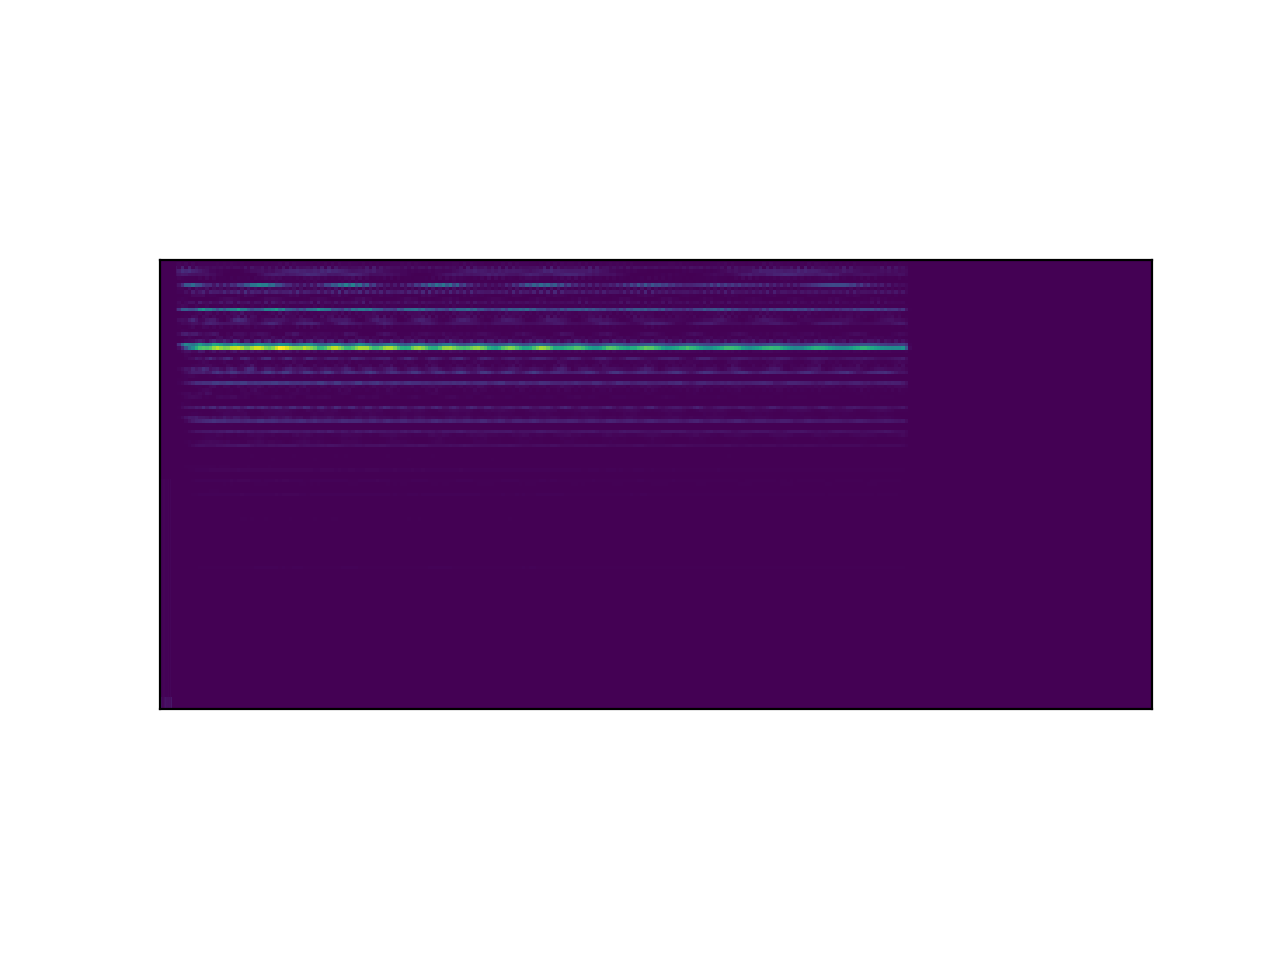
\includegraphics[width=.8\linewidth]{input.png}
  \caption{Input: The spectrogram of a given note, pitch\\ and velocity in Keyboard}
  \label{fig:sfig1}
\end{subfigure}%
\begin{subfigure}{.5\textwidth}
  \centering
  
\includegraphics[width=.8\linewidth]{out.png}
  \caption{Output: The spectrogram produced by our network for the input}
  \label{fig:sfig2}
\end{subfigure}
\begin{subfigure}{.5\textwidth}
  \centering
  
\includegraphics[width=.8\linewidth]{exp_out.png}
  \caption{Expected output: The spectrogram of the same\\ note, pitch and velocity in Mallet}
  \label{fig:sfig2}
\end{subfigure}
\caption{Preliminary Results}
\label{fig:results}
\end{figure}

\section{Timeline}
An approach we plan to explore is to train separate auto-encoder networks for mallet and keyboard. To translate from keyboard to mallet, a possible approach is to encode using keyboard and decode using mallet. Independently training the networks might not work as they may be of different scales. We want to look into some sort of combined training of these networks. 
We plan to learn more about CNNs and associated techniques, and then propose a few CNN-based auto-encoders whose design is better tailored for extracting instrument information from single-pitch spectrograms. 
We also want to look into extending this approach to longer audio clips. A possible approach that we plan to explore is to divide them into smaller chunks, do the style transfer and them combine them smoothly. 
All the three of us will be working on these together and plan to achieve our goal of converting audio from one instrument to another before the final week.

\pagebreak

\bibliographystyle{plain}
\bibliography{references.bib}

\appendix

\section{Network Architecture}

To get a baseline, we created an encoder-decoder network from just fully-connected layers and ReLu activations.  Going from outside in, the encoding layers consist of 256, 128, 64, 32, and 16 hidden units, and the same number of units in reverse (increasing) order for the decoding layers. We finally include a a fully-connected output layer with number of units equal to our input spectrogram shape, so that we may compute the loss function. We used Adam optimizer with a learning rate of $0.001$. We trained the autoencoder using keyboard dataset for 10,000 epochs.

\end{document}
